
%(BEGIN_QUESTION)
% Copyright 2006, Tony R. Kuphaldt, released under the Creative Commons Attribution License (v 1.0)
% This means you may do almost anything with this work of mine, so long as you give me proper credit

Determine the LRV and URV points for a transmitter measuring water level in this vessel, with the $\Delta$P transmitter elevated 10 feet above the vessel bottom and connected to it with capillary tubing and a remote seal filled with silicone fill fluid (SG = 0.934):

$$\includegraphics[width=15.5cm]{i00260x01.eps}$$

Also, explain why a remote seal is absolutely necessary in this installation.  It would not be a good idea to simply connect the ``high'' port of the $\Delta$P transmitter to the bottom of the vessel with a length of tubing as is permissible when the transmitter is either level with the bottom of the vessel or suppressed below the vessel's bottom!

\vskip 10pt

Be sure to show all your mathematical work so that your instructor will be able to check the conceptual validity of your technique(s).  A good way to check to see if you're solving the problem correctly is to check that each and every one of your intermediate calculations (i.e. the results you get mid-way during the process to arrive at the final answer) has real physical meaning.  {\bf If you truly understand what you are doing, you will be able to identify the correct unit of measurement for every intermediate result and also be able to show where that number applies to the scenario at hand}.


\vskip 20pt \vbox{\hrule \hbox{\strut \vrule{} {\bf Suggestions for Socratic discussion} \vrule} \hrule}

\begin{itemize}
\item{} Demonstrate how to {\it estimate} numerical answers for this problem without using a calculator.
\item{} When calculating hydrostatic pressures, there are two common methods: one is to use the formula $P = \gamma h$ and another is to translate inches of vertical liquid height directly into PSI using the known relationship between water and PSI (1 PSI = 27.68 inches of water).  Demonstrate both methods applied to this problem.
\item{} A good problem-solving technique is to imagine (perform a ``thought experiment'') the {\it converse} of a given question.  Here, you were asked to explain why a remote seal is necessary.  Present a thought experiment where you envision the opposite condition (e.g. the {\it lack} of a remote seal), and explain how this might help you to answer the initial question.
\item{} Should the ``low'' side of the DP transmitter be vented or sealed?
\end{itemize}

\underbar{file i00260}
%(END_QUESTION)





%(BEGIN_ANSWER)

%(END_ANSWER)





%(BEGIN_NOTES)

Calculating the hydrostatic pressure created by the 10 foot capillary tube (alone) below the transmitter:

$$\left(-10 \hbox{ ft silicone} \over 1 \right) \left(12 \hbox{ in} \over 1 \hbox{ ft} \right) \left(1 \hbox{ PSI} \over 27.68 \hbox{ in WC} \right) \left(0.934 \hbox{ in WC} \over 1 \hbox{ in silicone} \right) = -4.049 \hbox{ PSI}$$

\vskip 10pt

A full tank of water will add another 40 feet worth of hydrostatic pressure to the transmitter's ``H'' port:

$$\left(40 \hbox{ ft WC} \over 1 \right) \left(12 \hbox{ in} \over 1 \hbox{ ft} \right) \left(1 \hbox{ PSI} \over 27.68 \hbox{ in WC} \right) = 17.341 \hbox{ PSI}$$

\vskip 10pt

When the tank is empty (LRV condition), the transmitter only sees the $-4.049$ PSI vacuum created by the $-10$ feet of silicone fill fluid.  When the tank is full (URV condition), the transmitter sees the $-4.049$ PSI {\it plus} the 17.341 PSI created by the 40 feet of water, the total pressure being 13.292 PSI.

\vskip 10pt

LRV = $-112.08$ "W.C. = $-4.049$ PSI

\vskip 10pt

URV = +367.92 "W.C. = 13.292 PSI

\vskip 10pt

If no remote seal is present, liquid normally filling the instrument tube may dribble out when the vessel's level is low.  This would cause the static pressure of the impulse line to change, thus shifting the zero (LRV) of the transmitter.

\vskip 10pt

We may simulate the vacuum condition by applying a positive test pressure of 112.08 "W.C. to the {\it low} port of the $\Delta$P transmitter.

%INDEX% Measurement, level: hydrostatic pressure (elevated zero)

%(END_NOTES)


